\section{ATLAS Detector Upgrade}

\subsection{High Luminosity Large Hadron Collider - HL-LHC}
The Large Hadron Collider (LHC), run by CERN at the Franco-Swiss border near Geneva, is a circular accelerator with 27 km of acceleration pipes, is
the largest scientific instrument ever designed and built for scientific research. Successfully commissioned in March 2010 for proton-proton collision
with a 7 GeV centre-of-mass energy.\\ The LHC is pusshing the limits of human knowledge, enabling physicist to go beyond Standar Model (SM): the
enigmatic Higgs boson, mysterious Dark Matter and the world of supersymetry are just three of the long-awaited mysterous that the LHC will unveil. The
announcement given by CERN on 4 July 2012 about the discovery of new boson at 125-126 GeV, almost certainly the long awaited Higgs particle, is the
first fundamental discovery, hopefully the first of a series, that the LHC can deliver.\\ Such discovery was thanks to the different detectors located
on the four interaction points; ALICE, LHCb, CMS and ATLAS. This last one is the detector where our university is taking part.\par
\begin{figure}[ht]
		\centering
		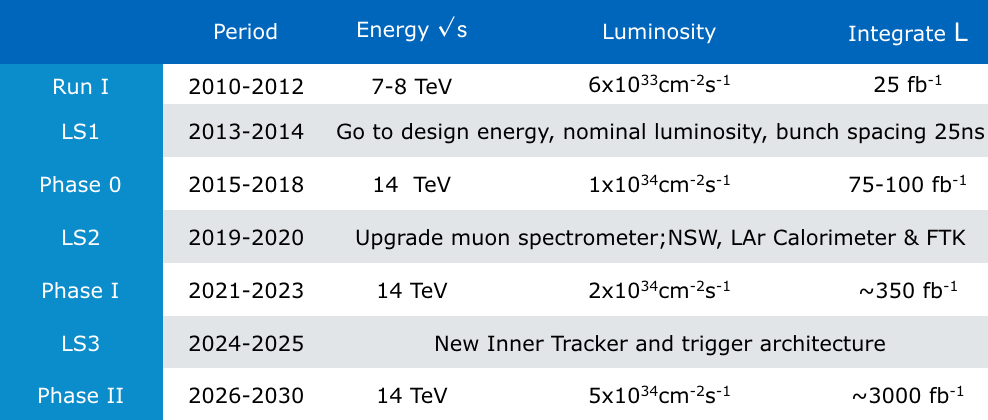
\includegraphics[width=0.7\textwidth]{LHC_program_table.png}
		\caption{LCH Schedule}\label{fig:a}
\end{figure}
\par
CONTINUE WITH LHC UPGRADE and GOALS

\subsection{ATLAS Detector}
The ATLAS detector it is a general-purpose detector, designed to explore proton-proton colissions at center of mass up to $\sqrt{s}=$14 GeV. Looking for.... \par
Such energy has been achived from 2015 and successfuly working with a luminosity of 1x10$^{34}$cm$^{-2}s^{-1}$ from 2016.\\

\textcolor{red}{Describe ATLAS detector and its part, together with the problem faced by now.
ENDING WITH THE FAKE TRIGGERS AND PROBLEMS FOR LOW PT.}



\subsection{New Small Wheel}

In manner to fullfill the LHC program (in fig.\ref{fig:a}), and in order to benefit from the expected high luminosity performance that will be provided by the
Phase-I upgraded LHC, the first station of ATLAS muon end-cap system (Small Wheel, SW) will need to be replaced.  The New Small Wheel (NSW) will have to operate
in a high background radiation region (upto 15kHz/cm$^2$) while reconstructing muon tracks with high precision as well as furnishing information for the Level-1
trigger. These performance criteria are demanding. In particular, the precision reconstruction of tracks for offline analysis requires a spatial resolution
about 100 \micro{m}, and the Level-1 trigger track segments have to be reconstructed online with an angular resolution of symroximately 1mrad. The NSW will have
to chamber technologies, one primarily devoted to the Level-1 trigger function (small-strip Thin Gap Chambers, sTGC) and one dedicated to precision tracking
(Micromegas detectors, MM). The sTGC are primarily deployed for triggering given their single bunch corssing identification capability. The MM detectors have
exceptional precision tracking capabilities due to their small gap (5mm) and strip pitch (symroximately 0.5mm). Such a precision is crucial to maintain the
current ATLAS muon momentum resolution in the high background environment of the upgraded LHC. The MM chambers can, at the same time, confirm the existence of a
track segments found by the muon end-cap middle station (Big Wheels) online. The sTGC also has the ability to measure offline muon tracks with good precision,
so the sTGC-MM chamber technology combination forms a fully redundant detector system for triggering and tracking both for online and offline functions. This
detector combination has been designed to be ablo to also provide excellente performance for the eventual High Luminosity LHC upgrade.\par 



\section{Small-strip Thing Gap Chamber}

The Small strip Thin Gap Chamber (a.k.a sTGC) detector it is a multi-wire proportional chamber (MWPC)  working in a high gain mode with a cathode-anode pitch
smaller than the anode-anode pitch, mostly based on the design of the Thin Gap Chamber\cite{tgc}, with thinner strips as the main improvement from the previous
version. The TGC tecnology has been used since 1988 in OPAL experiment and currently are part of the the muon spectrometer in ATLAS. \\ This new  chamber has
the advantage of having a 3.2mm strip width compare to the \textcolor{red}{5-6 mm} from the previous TGC, that is why it is called small strip Thin Gap
Chamber.\\ The size of the strips has been choosen to cope up with the precision resolution require for the NSW (explained before), where it has to be better
than 100 $\mu$m and provide a reponse with a few nanoseconds. For this purpose, chambers with different strips sizes has been build and test under pion beams,
chosed the 3.2mm has the best option\cite{stripwidth}. \par
%-------- sTGC Explanation -------

The sTGC is made of two resistive cathods planes, one with csymer strips and the other with pads, each cathode plane is made of FR4 with 1.6mm of thickness,
where  100 $\mu$m of csymer is etched for strips (pads) and then pressed with a 100 $\mu$m of FR4 over it and then sprayed with graphite to provide 100-200
k$\Omega / \square$ (1 M$\Omega/\square$ for TGC) so it can be treatead as a resistive cathode plane.\\ The anodes are golden tungsten wires of 50 $\mu$m
diameter, distributed at 1.8 mm between each other. The gas gap (2.8mm) is filled with a mixture of carbon dioxide (CO$_2$) and n-pentane(C$_5$H$_12$) in
proportion 55:45 respectively both strongly quenching gases that provide a high amplification factor and relatively low sensitivity to mechanical
variations.\textcolor{red}{[ref Mechanical variations]}\par  

%----------- How its produce the ionization and drifts  -----

%----------- sTGC mode picture -----

\begin{figure}[ht]
		\centering
		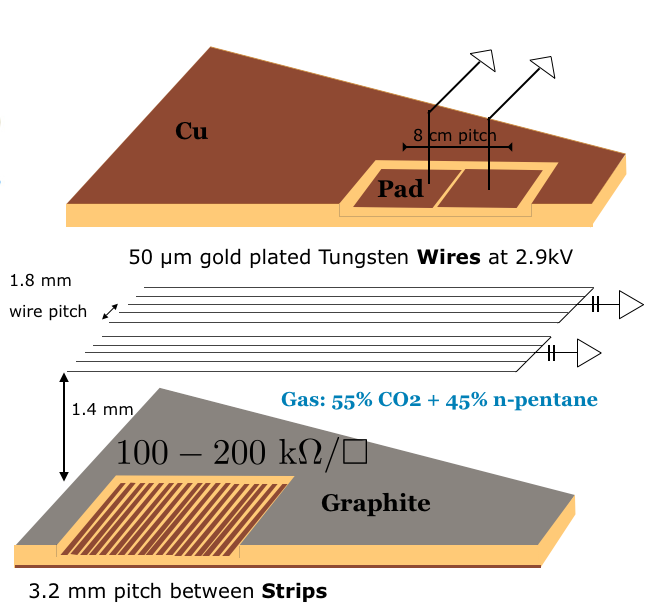
\includegraphics[width=0.5\textwidth]{sTGC_layout.png}
		\caption{Single plane sTGC}\label{fig:sTGC}
\end{figure}

A MWPC detector type  is a relativetely old technology, its succesfuly introduction to detector system in 1968 gave the Nobel prize to George Charpak in 1992.
This device has been a major ingrediente in detector systems since it can achieve spatial resolutions of 500 $\mu$m or less, and has typical time resolution of
about 30 ns.\\ The TGC has been built as a MWPC with a thinner gas gap, its means, the distance from the anode-cathode is smaller than the anode-anode (wire to
wire) to provide a fast time response, and at the same time giving a higher amplification, to achieve this smaller distance, precautions must be taken into
account when the internal pieces are construct, for that a precision of 50 $\mu$m must be achieve.\\ To work with such geometry several test were made to find
the proper gas mixture\cite{gaschoice}. Find the most suitiable mixture of  55\% well known carbon dioxide as a quenching gas, and a 45\% of n-pentane, which
for his nature can absorb energy in many ways of molecules  degree of freedom, vibrational, rotational, etc.\par 


\begin{itemize}
\item voltaje de operacion.
\item resitividad del graphito y para que usamos grafito.
\item Que es lo moderno de este detector...
\end{itemize}


\section{Construction process}
Since the main novelty on this detector is the high resolution obteined on xy plane due to the strip boards and the alignment between each chamber to get
precission about 50\micro m and 30\micro m respectively, its important to discuss how we achieve those numbers. Everything relies on how well are those chamber
built and also how the cathodes boards (strips and pads) are fabricated. The size of each chamber are around 1m$^2$ to 2m$^2$ and for the current fabricant it
is complicated to achieve 50 \micro m resolution etching a pcb board accross 1.5 m without taking into consideration that the standard size for pcb boards are
70 cm long.  The attempt of this sections is to give an idea how the sTGC Quadruplets are built, mostly on the first module 0 produce by UTFSM, which is the QS1
(Quadruplet Small sector, part 1).  Being the smallest detector to be produce for the NSW, has some pro and cons. The main cons is related to the posistion of
the QS1 inside the NSW, it is the closest one to the interaction point and for that it get the highest rate of particles. For the same reason the position
resolution is a key point and the response against high rate particles it is a must.  Some pros are related to the size of it, with approximetely 1m long and 55
cm the small side and 75 cm the large side of the trapezoidal shape, the sTGC QS1 can be handly without any problems, its 45 kg at the final step is easy to
manage between two people, and with almost 1m long, the etching of strips boards (2.7 mm strip width and 0.5 mm etch) can be achieve with 50 \micro m. 

\subsection{Quality Control of cathode boards}

The cathodes for the module0 were maid by an Italian company MDT, and since it was the first production, the review was done at their place.\\ The
thickness of the board is measured in 19 points around the perimeter with a micrometer. The values of theses measurments must be whithin 1.6 mm $\pm$25\micro
m,exceding this numbers lead to the partial rejection of the cathode boards, however if there is a single point deviation of less than $\pm$ 35\micro m about
the average, it could be used in combination with another cathode board that does not have the same local deviation. The raw data is found in appendix X.\par An
electrical test is donde with a multimiter, to check if there is any short between strips or pads depending on the cathode board.\par The last step and the most
important is the dimensional control: this must be perform on a flat surface (done on a granite table at the construction site), with 2 pins that match the
brass inserts on the cathode and using a special caliper above the cathode board the misalignment is measured. The caliper is an aluminuim ruler machining  with a precision of 30 \micro m
at 20 Celsius degrees  has the same strip pitch for the first and last five strips and to avoid any paralax the thickness is the edge for those strips is 1mm. Looking
with a lens glass around this point it posible to detect some misaligment between this two strips (caliper and cathode board). A photography is taken and
analize to calculate this misaligment. For such distance (about 1 m long) some precaution must be take, considering the expansion coeficient for both material.
machining with a precision of 30\micro m measure at 20 Celsius degrees.\par

%------- Photography strip cathode board measurement ------------ % 
\begin{figure}[ht]
	\centering
	\hfill
	\begin{subfigure}[b]{0.35\textwidth}
		\centering
		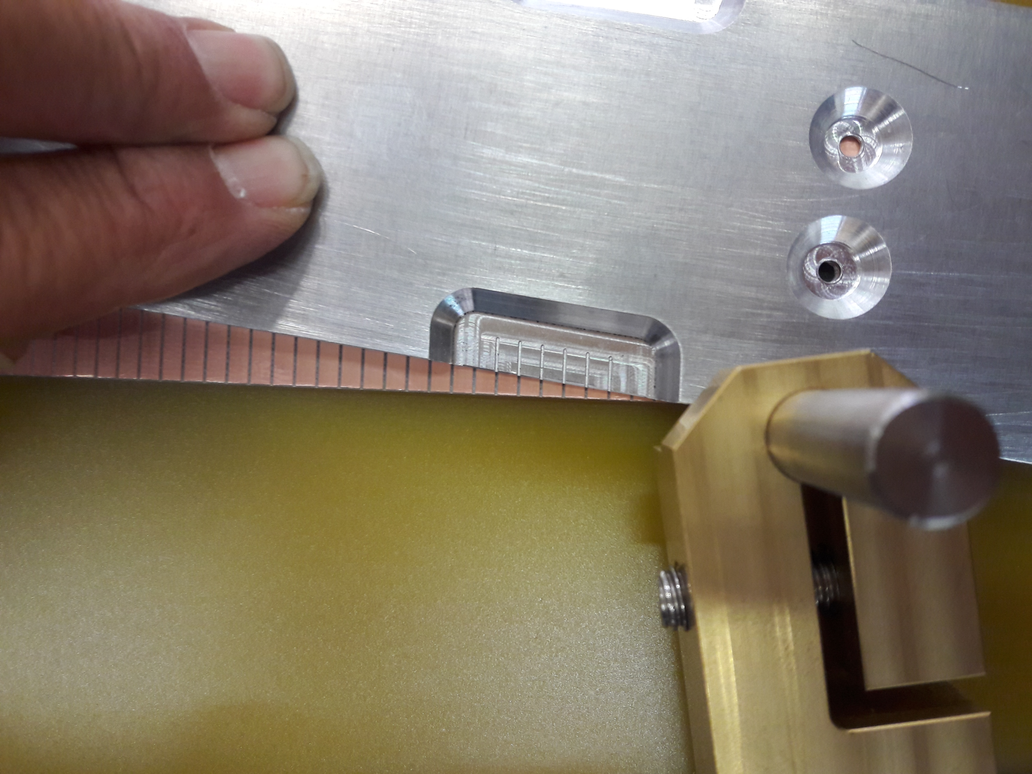
\includegraphics[width=\textwidth]{alignment.png}
		\caption{Al ruler used to check shift over the last strips.}
		\label{fig:ruler}
	\end{subfigure}
	\hfill
	\begin{subfigure}[b]{0.35\textwidth}
		\centering
		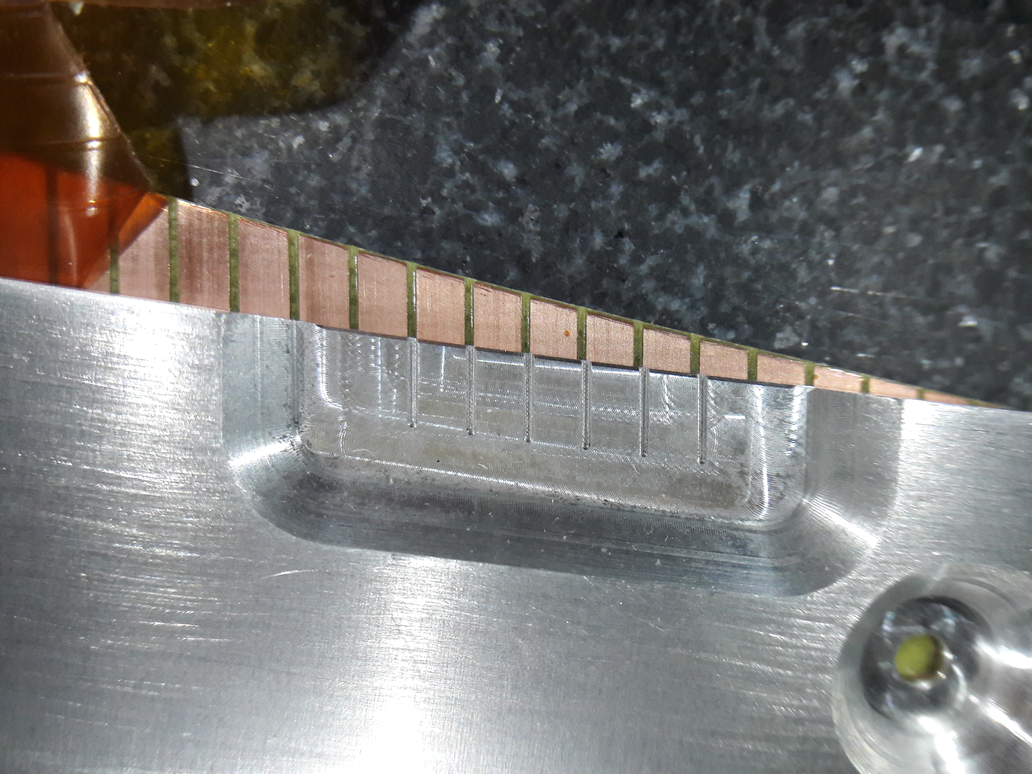
\includegraphics[width=\textwidth]{zoom_in.png}
		\caption{Zoom-in Comparing strip position}
		\label{fig:zoom}
	\end{subfigure}
	\hfill
\end{figure}

\subsection{Cathode preparation}
Once the cathodes pass all the dimensional control are cleaned with Acetone and Isopropyl acohol and placedplaced on a granite table with a flatness of better
than 30\micro m, and a vacuum system underneath and fixed on the edges with metal jigs which also has marks for the internal wire support or chamber section.
The places which does not be sprayed with graphite, like the wire support and the edges are covered with a \unit{3.5}{mm} black tape to  the designated wire
support locations across the board, and a blue tape the edges preventing spray graphite on the places where they will be glue. 

\subsection{Graphite spraying}
A key point for this process is to prepare the 'painting' a mixture of Graphite-33 with Plastik-70 bonding agent. The graphite must be agitated for at least 2
hours before mixing with Plastik-70. A proper ratio of 1500g Graphite and 540g Plastik is mixed for 20min before spraying.\par
A spraying machine is in charge to get this process done, meanwhile a temperature and humidity must be controlled. After the cathode is painted the superficial
resistance is measured on the edges and values above \unit{100}{k$\Omega/\square$} must get otherwise the cathode needs to be sprayed again.\par


\subsection{Polishing}
In manner to ensure an uniform resistivity across the chamber, the cathode is visually divide in 5x6 squares. Inside each square t
e resistivity is measure in 5
to 7 points with a probe and simultaneously brush it in the orientation that the wires will be wound. The brush must be done carefully without over-polish areas
because onces resistance drops down nothing will bring it back up. 


\subsection{Glue internal parts}
After removing all the blue and black tape, all the internal parts such buttons to provide mechanical support to the gas gap, the wire support which help them
to not bend due to gravity and create catenary effect, and all the external frames to provide the \unit{1.4}{mm} height for the gas gap. All this part are
cleaned with isopropyl alcohol, meanwhile the glue, a type of epoxy (2011-Araldite) is prepare. This glue will not only fix the part, also will fill the
surfaces where those part are had less thickness than is requested.


\subsection{Winding wires}
A flat table which can spin around on one axis is used to winding the cathodes board. On each side of the table one cathode with all the internal parts
previosly glued is mounted and tight it with metal clamps on the edges, meanwhile a vacuum is apply underneath to ensure the flatness of the cathode.
A winding machine is in charge of this process, taking all the precautions to place every wire at \unit{1.8}{mm} between each other with \textcolor{red}{\unit{50}{\micro
m} precision?}.\\
After the process is done, all the wires are solderd in group of 10 in the wire rulers with \unit{10}{M$\Omega$} resistor to the high voltage line, later on the
remaining wire can be cut and the metal clamps around the edges can be removed. 


\subsection{Detector Assembly}

Once the Pad cathode board with all wires soldered is cleaned with clean water and dry with clean air. The board is place on the granite table, vacuum is
applied underneath so it can be ready to connect it to high voltage. It is necessary to monitor the current from the cathode meanwhile the voltage is increased,
starting with 100V and reach 3000V, every 100V step the current is monitoring and check that never goes higher than \unit{1}{\micro A}, if it is the case, the
cathode needs to watch carefully on each corner to see some small sparks around dust or remaining glue from the previous process.\\
Reaching the nominal current, the strip cathode board is placed against the pad cathode board carefully, and an aluminuim frame with a sillicon rubber is placed
on top to isolate the chamber from the environment, afterwards the vacuum is applied to this chamber and only CO2 is flushing inside the chamber. Now it is the
time to turn on the power supply and watch if there is no sparks (monitoring the current), if it is not the case, the glue is prepared to close the chamber
inmediataly to prevent any dust enter the chamber when the sillicon ruber and the strip cathode board is remove. Finishing this process, a \underline{single chamber
detector is considered done}.\\
Closing two chambers is possible build a doublet, for that it is necessary to glue a honeycomb with a well known thickness (\unit{5$\pm$0.02}{mm}) 


\subsection{Planarity and thickness measurements}
Total thickness.

\section{Gain uniformity measurements}

After the chambers are built it is important to know the response of the detector, and a primitive way to do such thing without any electronic readout attach
to strips or wires, is to measure the current draw from the power supply and see how it behaves to a radiation source.\\ There are two ingredients that can
produce gain variations on wire detectors, the first one is the \'nature" gain fluctuations from the charge production in proportional counters which follow
Polya distribution, however is less pronounced in semi-proportional mode such as sTGC working region.\\ The second one is related to the mechanical tolerances,
this part is very well known since 40 years as it is presented on Sauli's book about drift chambers and tell us that for a diameter variations of the wire about
1\% (fabrication precision) will result on a 3\% change in the gain, where as about \unit{100}{$\mu$m} difference in the gas gap thickness (\unit{2.7}{mm})
results in about 15\% change of the gain. The effect of a wire displacement of about \unit{100}{$\mu$m} of a wire plane results in 1\% int the charge of the two
adjacent wires which with a gain of $\sim10^6$ will give a $\sim10\%$ change in the gain.\\ Taking all of this in consideration is expected to get a gain variation less
than 20\% as Quality Acceptance.\\ In this test the gain is considered as the current draw measured from the power supply and its need to test under two
different working points (bias voltage), one when the chamber it is not in the limited proportional region, 2500 volts, a take it as a reference compare to the
2900 volts which is the operational voltage.\par

%-------- why x ray source ? ----------
For such test the x-ray source is used due to the many advantages:\par
\begin{itemize}[noitemsep, topsep=0pt, parsep=0pt, partopsep=2pt]
	\item Mostly mono-energetic photons.
	\item Variable current: which can provides different rates. [\unit{1}{$\mu$A} - \unit{200}{$\mu$A}]
	\item Variable voltage: modifying breaking voltage of electrons inside the x-ray gun. [\unit{10}{keV} - \unit{50}{keV}]
	\item Different spot size: with a set of collimator it is possible to irradiate only interesting area.
	\item Portable, it is possible to move across the sensitive area of the detector.
\end{itemize}


\subsection{Setup}
To perform such test a x-ray gun called Mini-x from Amptek is used, with silver (Ag) as transmission target with a beryllium (Be) end window is used.
Working under \unit{50}{kV} with \unit{45}{$\mu$A}, the emission spectra Fig.\ref{fig:minixgun} show two main photo peaks with 22 and 25 keV. The
aperture emissions is about 120 degrees, so a collimator of 5 degrees is placed to provide a spot size of \unit{4}{mm}.\\ The gun is mounted on a
robot arm KUKA, to move it across the detector irradiating a long the wires. Since the high voltage power supply give us a current average per
second, the vertical and horizontal step can be adjust to perform a spot size of 4$mm^2$ however the Mini-x device had some overheat issues so a
\unit{5}{cm} vertical step was chosen to perform a full irradiation test in less time. A more suitable step would be \unit{1}{cm} to detect
internal structures of similar sizes. The horizontal step was \unit{1.5}{cm}, enough to change completely from group wires, although it will better
to improve the granularity it is not possible since the issue explained before.
\begin{figure}[ht]
	\centering
	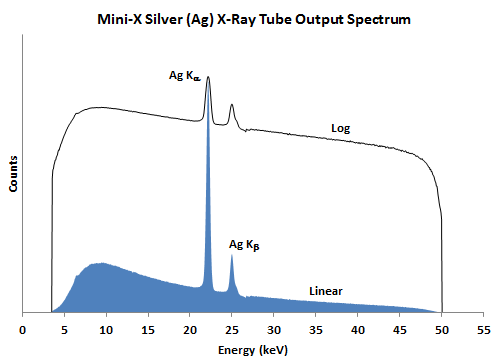
\includegraphics[width=0.5\textwidth]{minix_ag_1.png}
	\caption{X-ray emission spectra from Mini-X gun}\label{fig:minixgun}
\end{figure}

The irradiation test is taken in approximately one hour and the four chamber are done at the same time, meanwhile the division of each chamber are
connected to the same HV channel. 
\subsection{Results}
The next two set of histograms shows the distribution of the current draw at two different voltage, one at 2500V to take it as  reference since the cahmber can
be consider with no gain (no proportional mode), and the second one the voltage at what our chamber must be working 2900V.\\
On the Figure \ref{fig:2500V} an average of approximately \unit{200}{nA} can be observe on the four layers, considering \unit{50}{nA} when no source is present
(leakage current).
As previously discuss the important part is to get how uniform are the chambers across the whole sensitivity area, even the places where the internal parts are
found, such a wire supports and buttons, which in that case a notoriously decrease of gain (less current draw) is expected due to the lack of gas volume, and so
no amplification.\\
On the Fig\ref{fig:2900V} the current draw for each single chamber is shown with uniformity less than 17\%. Definitely improve the uniformity if only the places without wire
support are removed, having a XX\%.
\begin{figure}[hb]
	\centering
	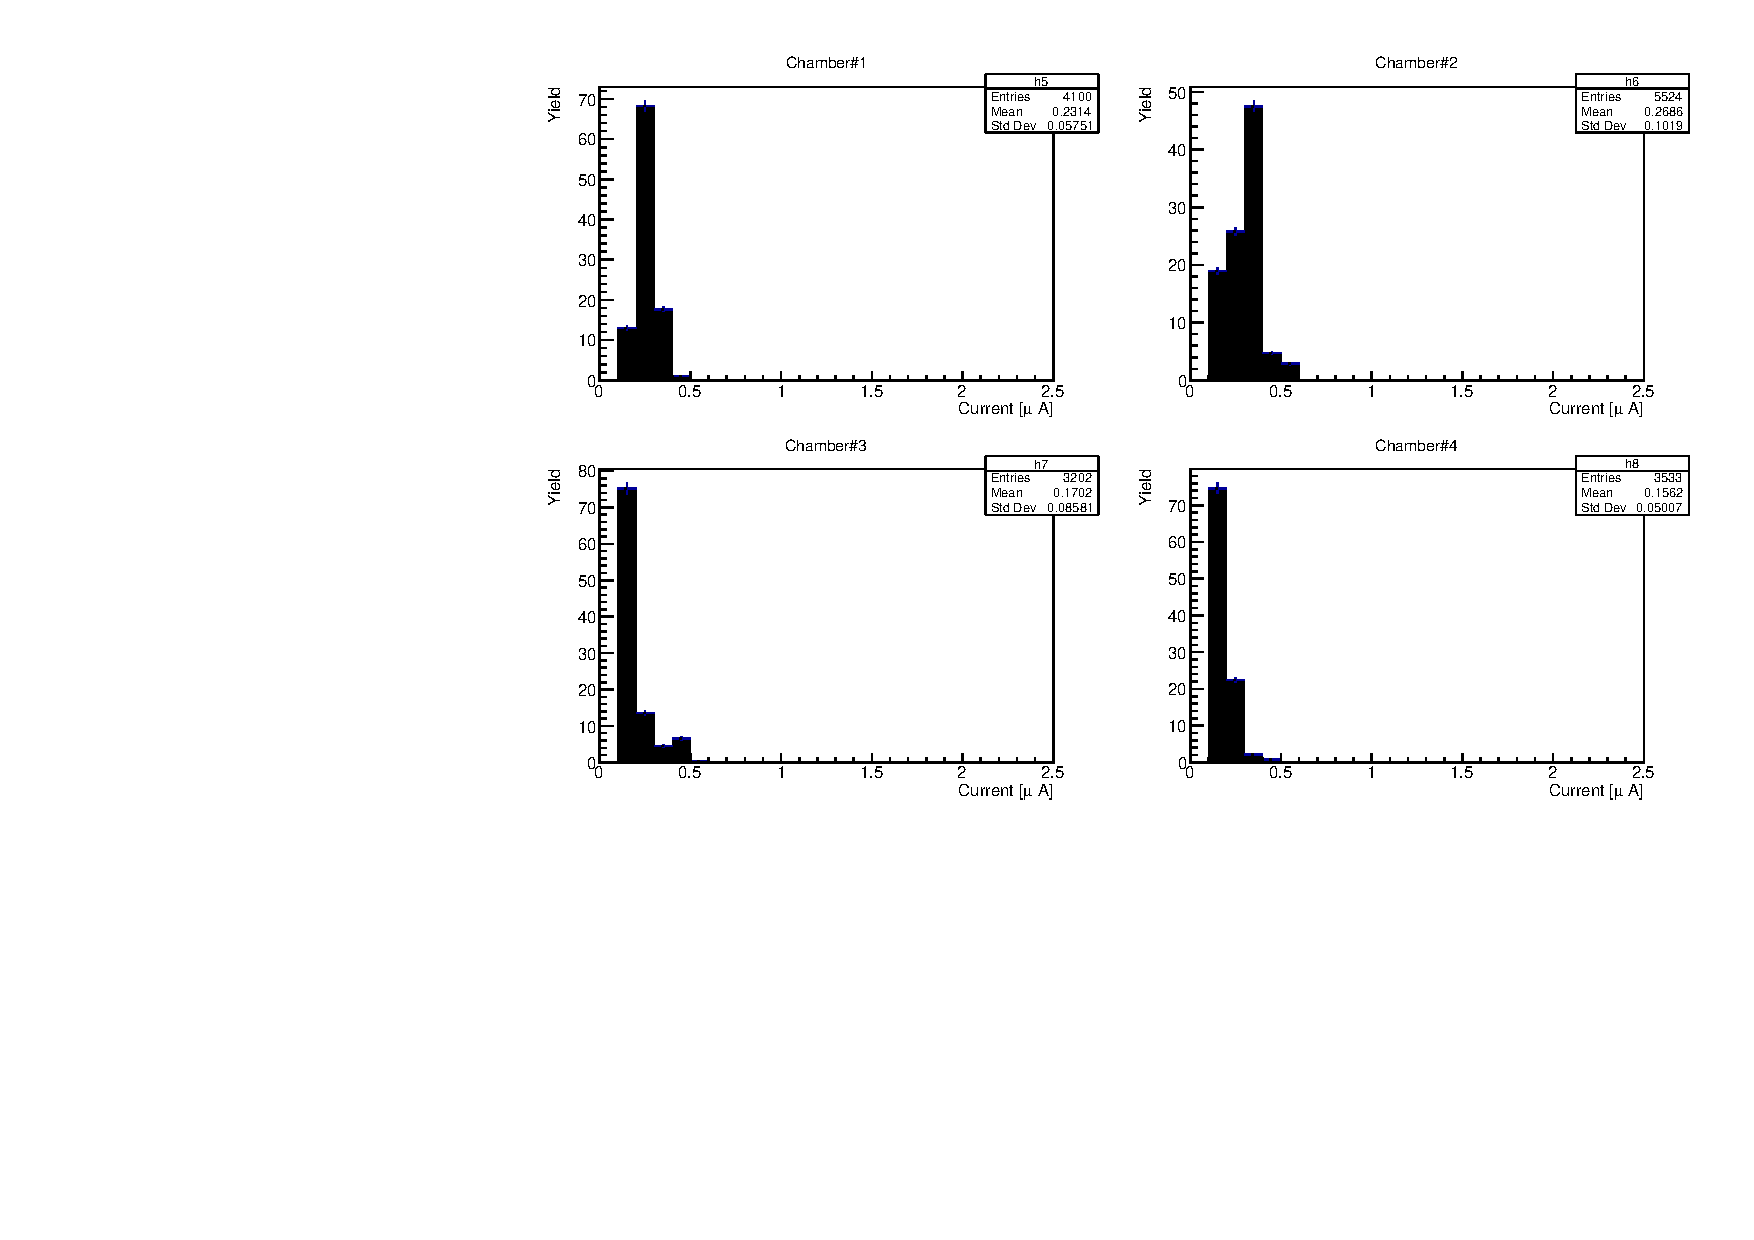
\includegraphics[width=0.8\textwidth]{uniformity_2500.pdf}
	\caption{Current from power supply at 2500V}\label{fig:2500V}
\end{figure}

\begin{figure}[ht]
	\centering
	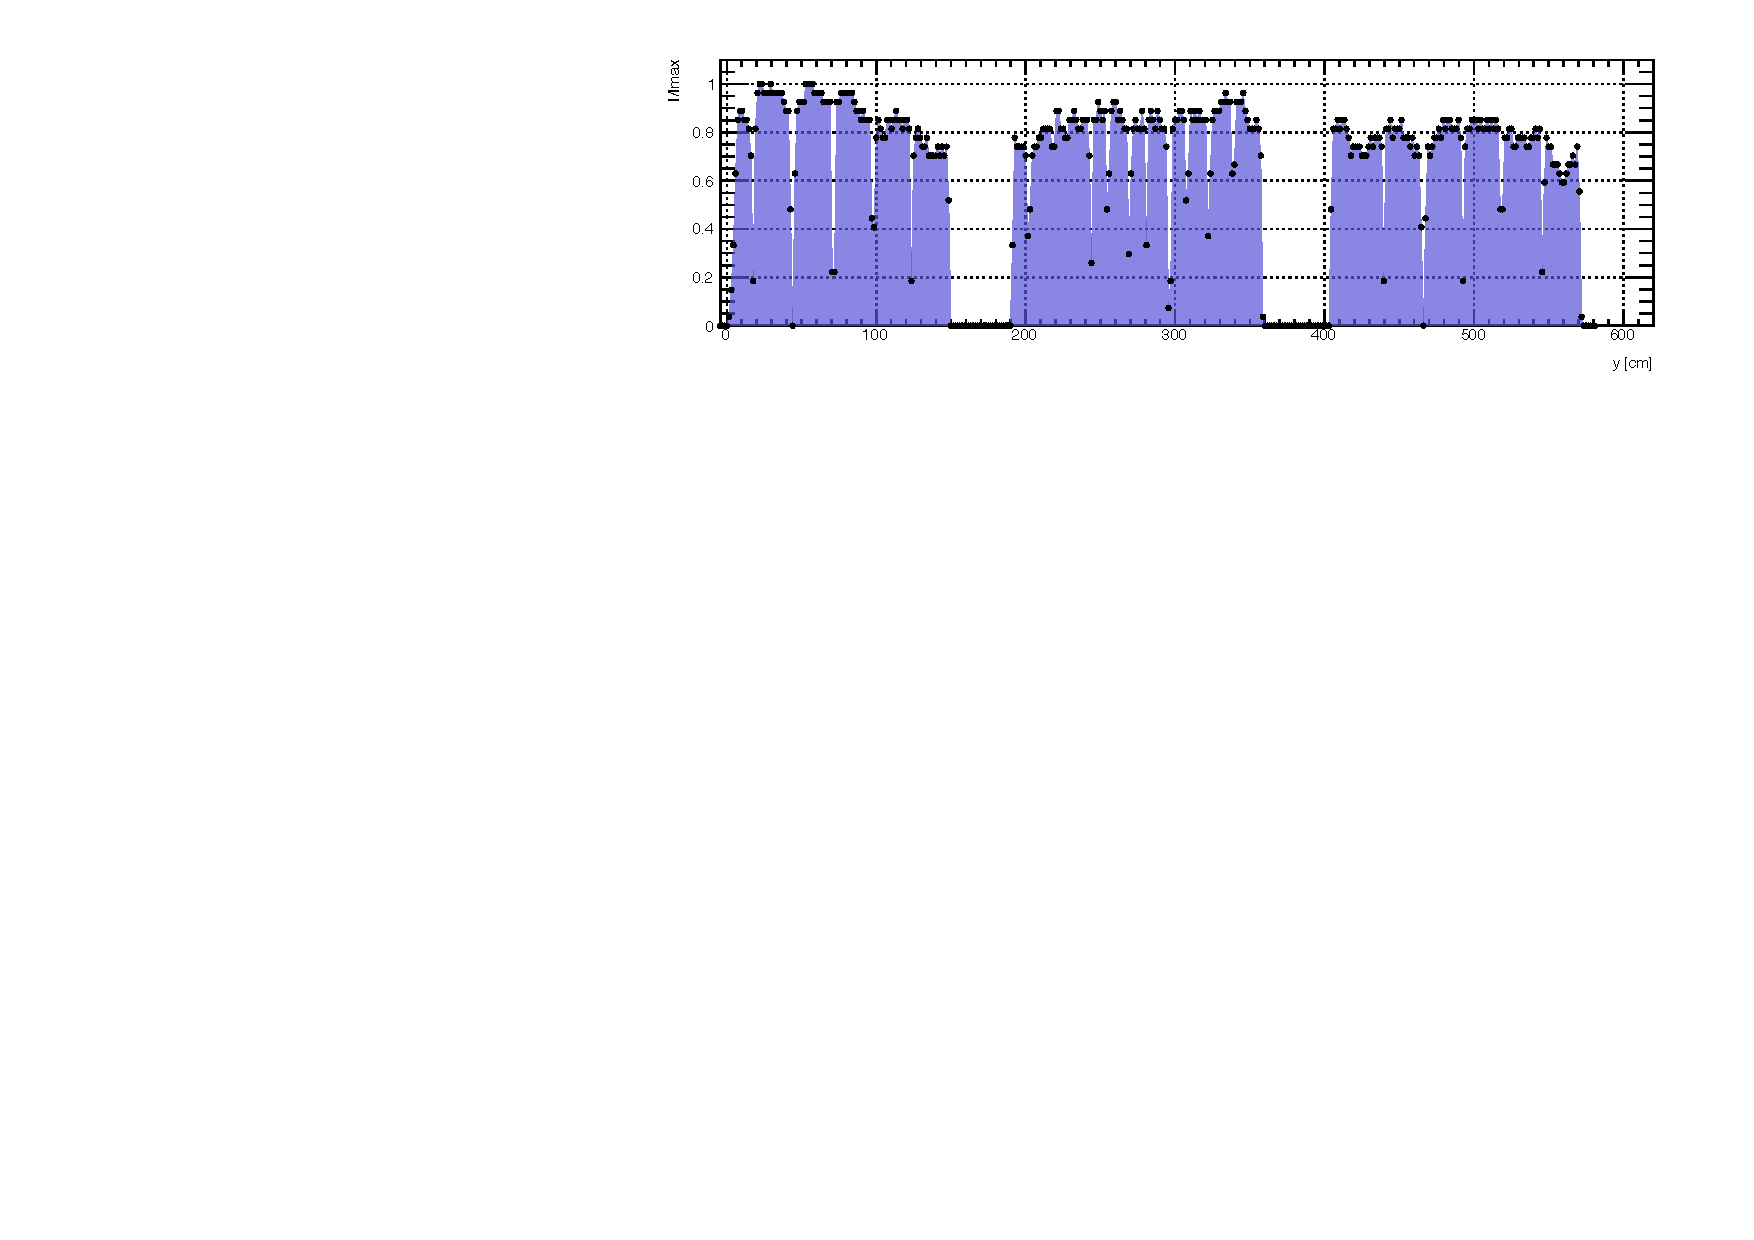
\includegraphics[width=0.8\textwidth]{uniformity_2900.pdf}
	\caption{Current from power supply at 2900V}\label{fig:2900V}
\end{figure}


\section{Test under high rate}


One of the key feature of this detector is to be able to work under different particles rates, and if it is capable of handle rates higher than
\unit{15}{kHz/cm$^2$}. For this Test of module0 inside of GIF++, together with rate measurement with small TGC monitor. 
Detector test under different atteuation filters.

\begin{figure}
	\centering
	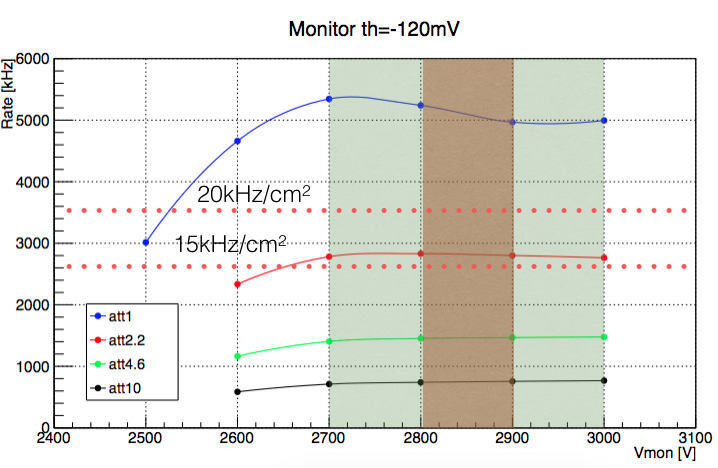
\includegraphics[width=0.7\textwidth]{monitor.png}
	\caption{Monitor rate}
	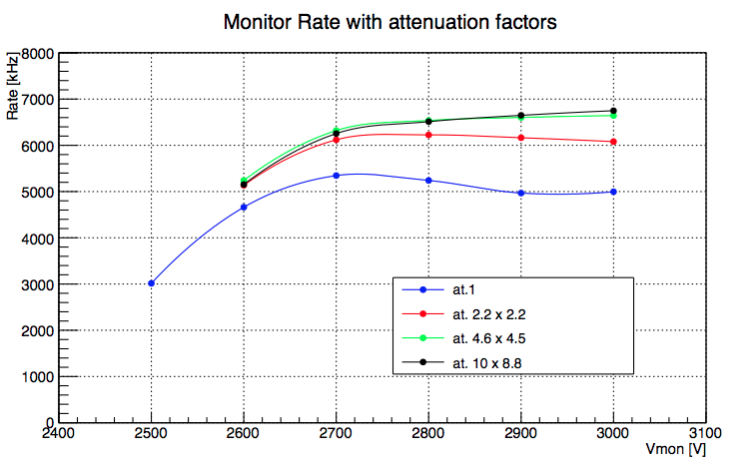
\includegraphics[width=0.7\textwidth]{rate_filters.png}
	\caption{Filters applied}
\end{figure}

\section{Spatial resolution strips}
\newpage
\section{Charge sharing between pads}
\newpage
\section{summary}
